\documentclass[11pt]{article}

% ------
% LAYOUT
% ------
\textwidth 165mm %
\textheight 230mm %
\oddsidemargin 0mm %
\evensidemargin 0mm %
\topmargin -15mm %
\parindent= 10mm

\usepackage[dvips]{graphicx}
\usepackage{multirow,multicol}
\usepackage[table]{xcolor}

\usepackage{amssymb}
\usepackage{amsfonts}
\usepackage{amsthm}
\usepackage{amsmath}

\usepackage{subfigure}

\graphicspath{{./pix/}} % put all your figures here.

\begin{document}
\begin{center}
\Large{\textbf{ECE 595: Homework 1}}

Yi Qiao, Class ID

(Spring 2019)
\end{center}


\subsection*{Exercise 2}
\noindent\textbf{(a)} For a guassian distribution:

\begin{equation} \label{eq1}
\begin{split}
E[x] &=\int_{-\infty}^{\infty}x\frac{1}{\sqrt{2\pi\sigma^2}}e^{-\frac{(x-\mu)^2}{2\sigma^2}}dx \\
	&=\int_{-\infty}^{\infty}(x+\mu)\frac{1}{\sqrt{2\pi\sigma^2}}e^{-\frac{x^2}{2\sigma^2}}dx \\
	&=\int_{-\infty}^{\infty}x\frac{1}{\sqrt{2\pi\sigma^2}}e^{-\frac{x^2}{2\sigma^2}}dx+\int_{-\infty}^{\infty}\mu\frac{1}{\sqrt{2\pi\sigma^2}}e^{-\frac{x^2}{2\sigma^2}}dx \\
	&=0+\mu\frac{1}{\sqrt{2\pi\sigma^2}}\times\sigma\sqrt{2\pi} \\
	&=\mu
\end{split}
\end{equation}
\begin{equation} \label{eq2}
\begin{split}
Var[x] &=\int_{-\infty}^{\infty}(x-\mu)^2\frac{1}{\sqrt{2\pi\sigma^2}}e^{-\frac{(x-\mu)^2}{2\sigma^2}}dx \\
	&=\frac{1}{\sqrt{2\pi\sigma^2}}\int_{-\infty}^{\infty}x^2e^{-\frac{x^2}{2\sigma^2}}dx \\
	&let\ y = \frac{x}{\sigma},\ then\ dy=\frac{1}{\sigma}dx \\
	&=\frac{\sigma^3}{\sqrt{2\pi\sigma^2}}\int_{-\infty}^{\infty}y^2e^{-\frac{y^2}{2}}dy \\
	&=\sigma^2
\end{split}
\end{equation}

\noindent\textbf{(b)} Data generated and plotted as follows.
\begin{figure}[h]
\centering
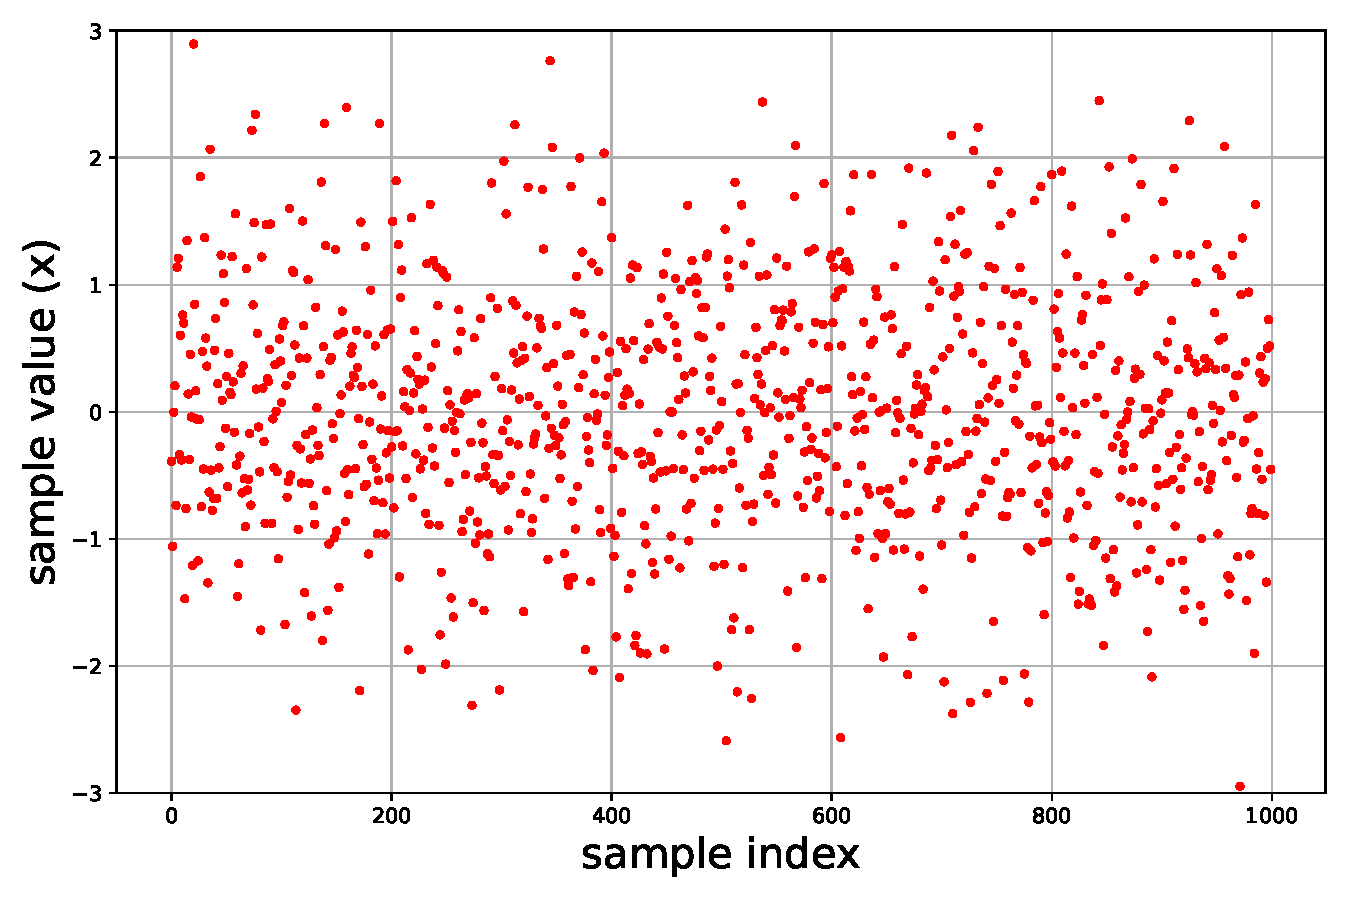
\includegraphics[width=0.5\linewidth]{exercise2_b}
\caption{Gussian random data.}
\label{fig: figure 1}
\end{figure}
\pagebreak

\noindent\textbf{(c)} \\
\textbf{(i)..(iv)} plots shown below

\begin{figure}[h]
\centering
\subfigure[4 bins]{
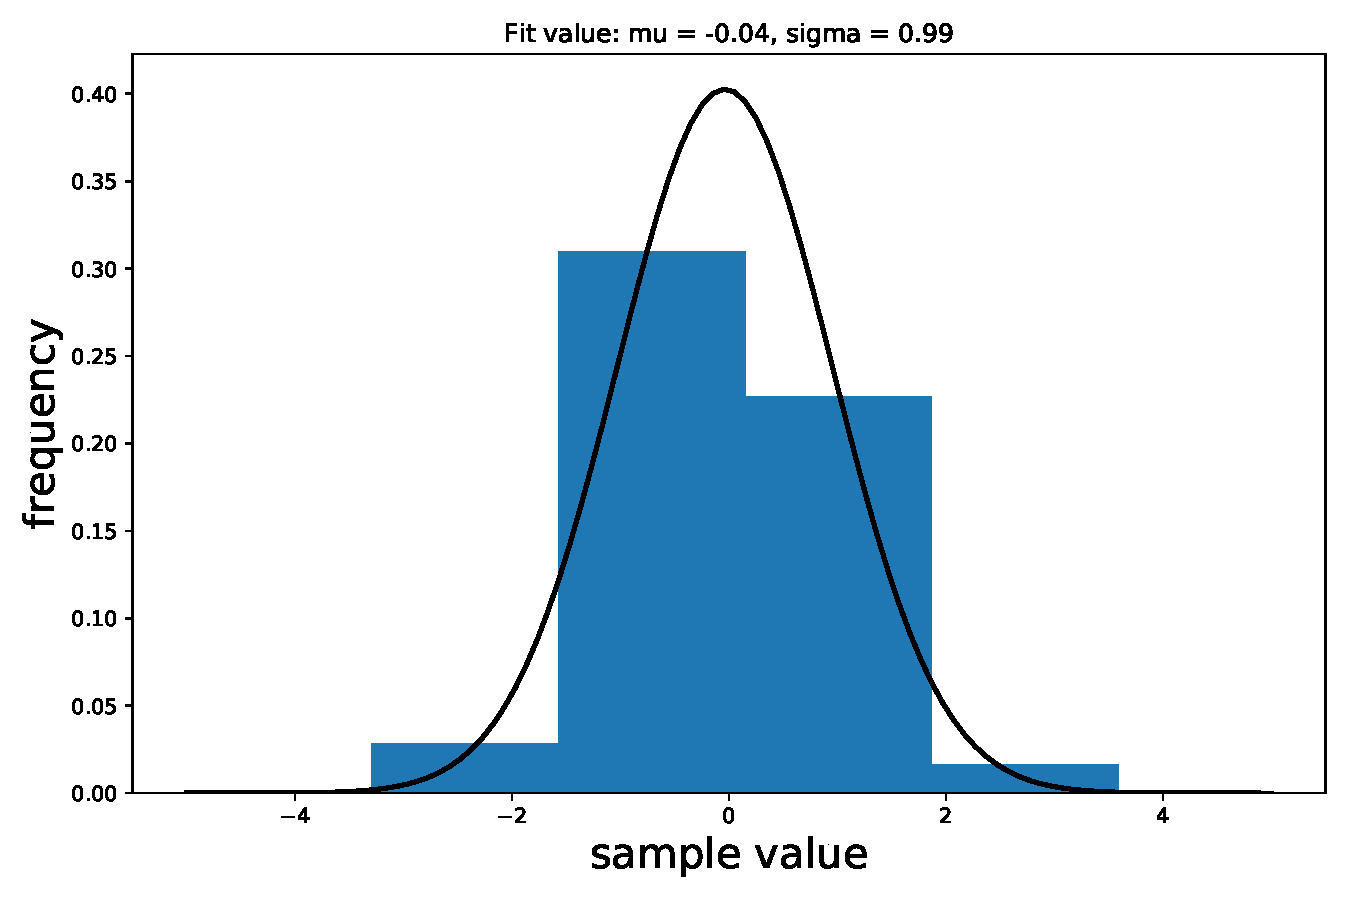
\includegraphics[width=0.47\linewidth]{exercise2_c1}
}
\subfigure[1000 bins]{
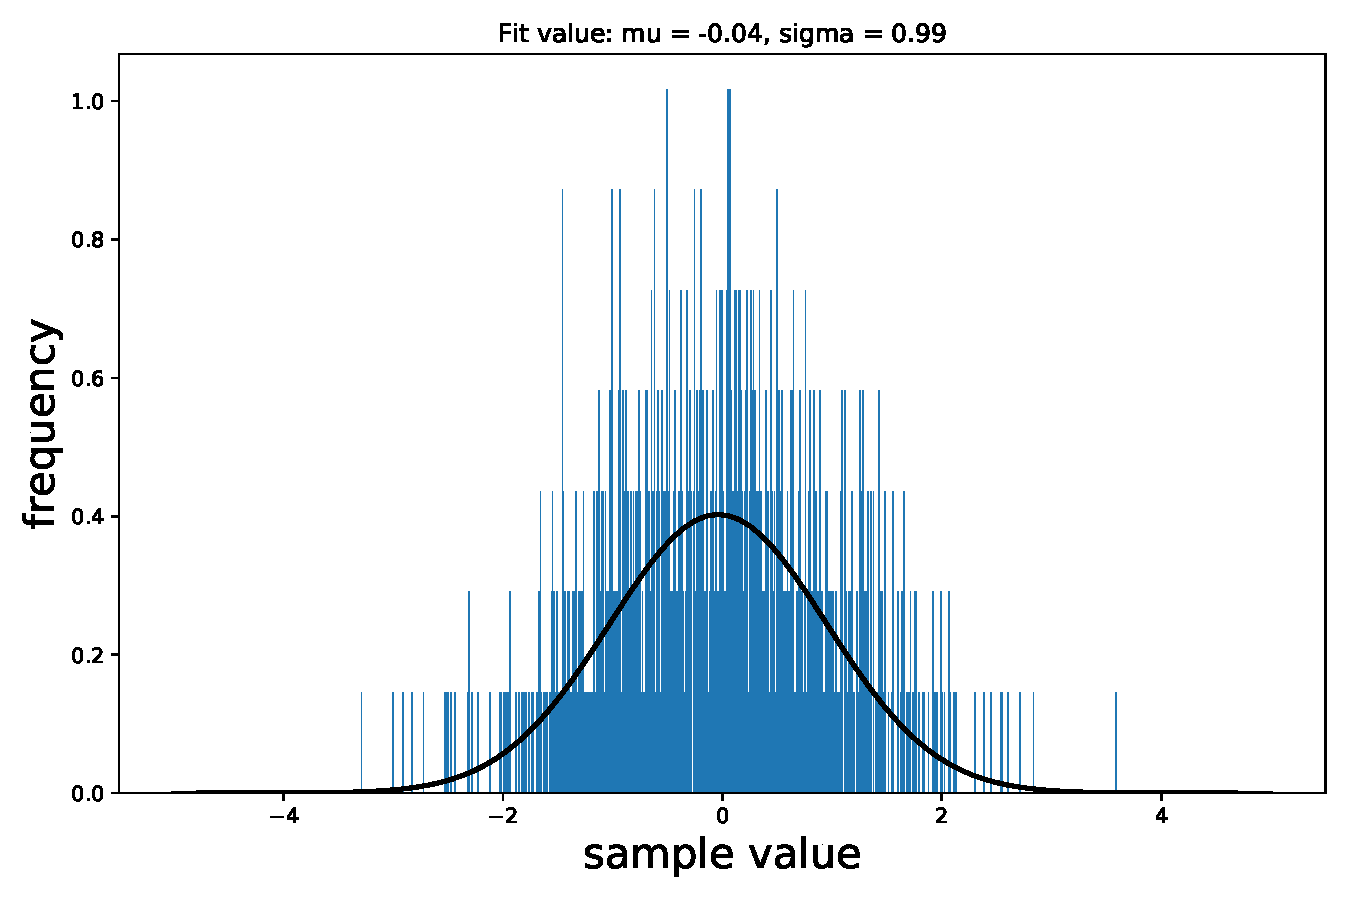
\includegraphics[width=0.47\linewidth]{exercise2_c2}
}
\end{figure}

\noindent\textbf{(v)}
TODO: fill this\\

\noindent\textbf{(d)}
compare to part (c), the histogram fits a lot better with the PDF
plots shown below

\begin{figure}[h]
\centering
\subfigure[Cross validation estimator of risk vs. \# of bins]{
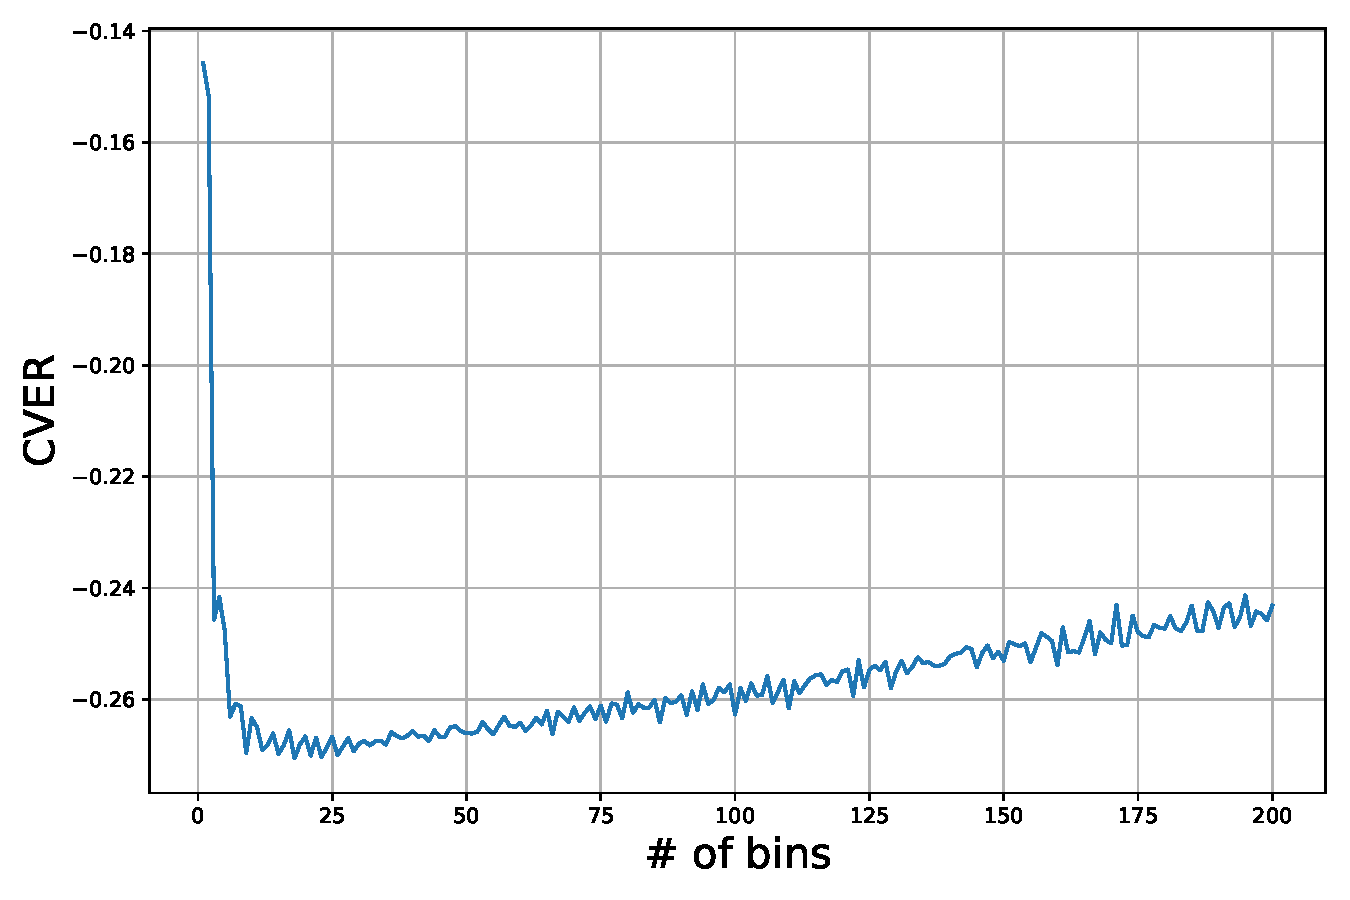
\includegraphics[width=0.47\linewidth]{exercise2_d1}
}
\subfigure[Histogram and PDF overlayed with optimized number of bins]{
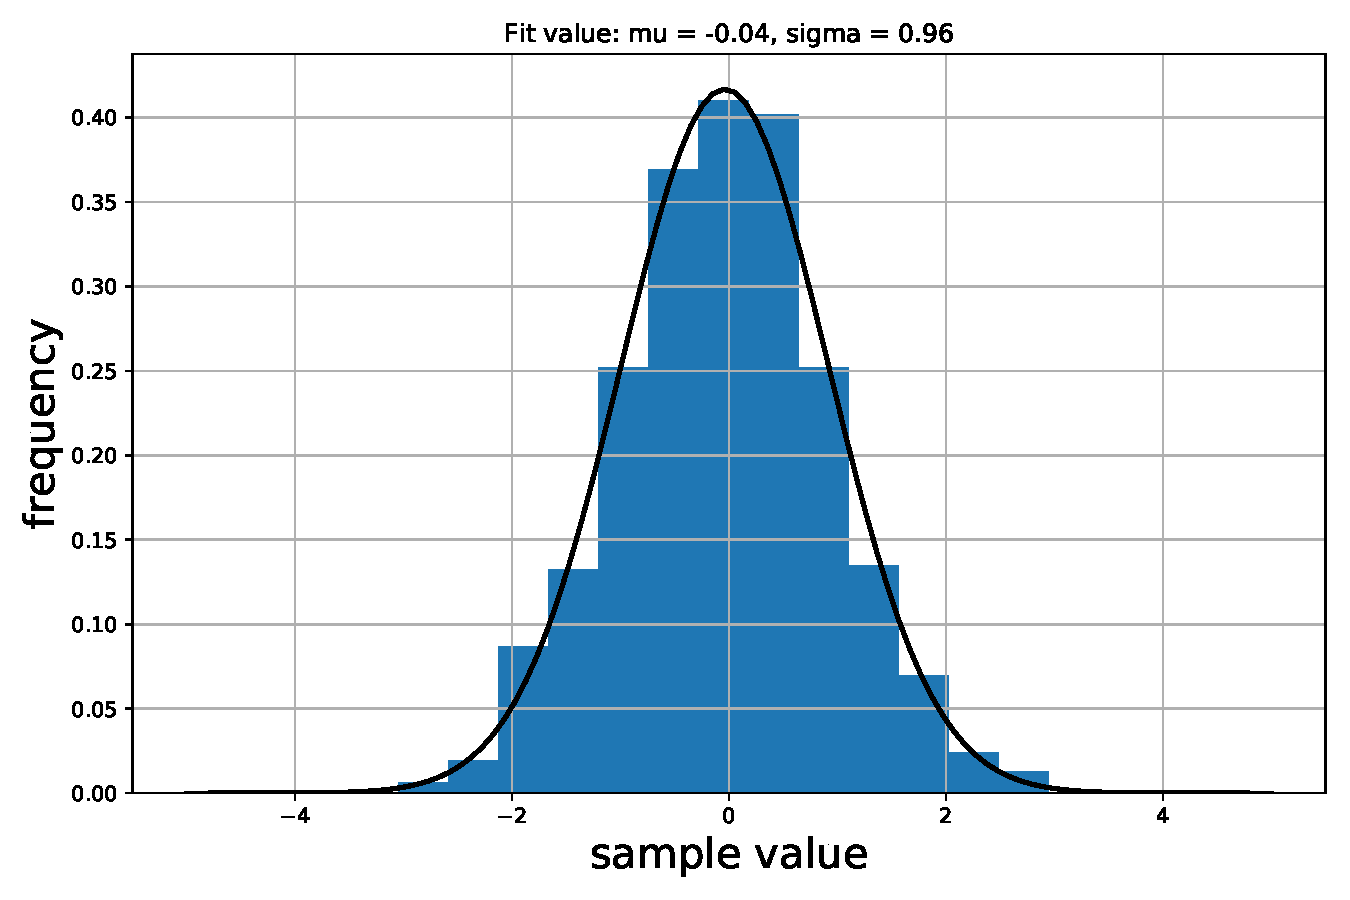
\includegraphics[width=0.47\linewidth]{exercise2_d2}
}
\end{figure}

\subsection*{Exercise 3}

\noindent\textbf{(a)}
$$f_\textbf{X}(\textbf{x})=\frac{1}{\sqrt{2\pi^2|\pmb{\Sigma}|}}exp\{-\frac{1}{2}(\textbf{x}-\pmb{\mu})^T\pmb{\Sigma}^{-1}(\textbf{x}-\pmb{\mu})\}$$

\noindent\textbf{(i)}
plug in\\

\begin{center}
$\textbf{X}=\begin{bmatrix} X_1 \\ X_2 \end{bmatrix}$, 
$\textbf{x}=\begin{bmatrix} x_1 \\ x_2 \end{bmatrix}$,
$\pmb{\mu}=\begin{bmatrix} 2 \\ 6 \end{bmatrix}$,
  and  $\pmb{\Sigma}=\begin{bmatrix} 2 & 1 \\ 1 & 2 \end{bmatrix} $
\end{center}

we get\\
\begin{equation}
\begin{split}
f_{\begin{bmatrix} X_1 \\ X_2 \end{bmatrix}}\left(\begin{bmatrix} x_1 \\ x_2 \end{bmatrix}\right)&=\frac{1}{\sqrt{2\pi^2\begin{vmatrix} 2 & 1 \\ 1 & 2 \end{vmatrix}}}exp\left\{-\frac{1}{2}\begin{bmatrix} x_1-2 \\ x_2-6 \end{bmatrix}^T\begin{bmatrix} 2 & 1 \\ 1 & 2 \end{bmatrix}^{-1}\begin{bmatrix} x_1-2 \\ x_2-6 \end{bmatrix}\right\}\\
&=\frac{1}{\pi\sqrt{6}}exp\left\{-\frac{1}{3}\left((x_1-2)^2-(x_1-2)(x_2-6)+(x_2-6)^2\right)\right\}\\
\end{split}
\end{equation}
\pagebreak

\noindent\textbf{(ii)}
plot shown below
\begin{figure}[h]
\centering
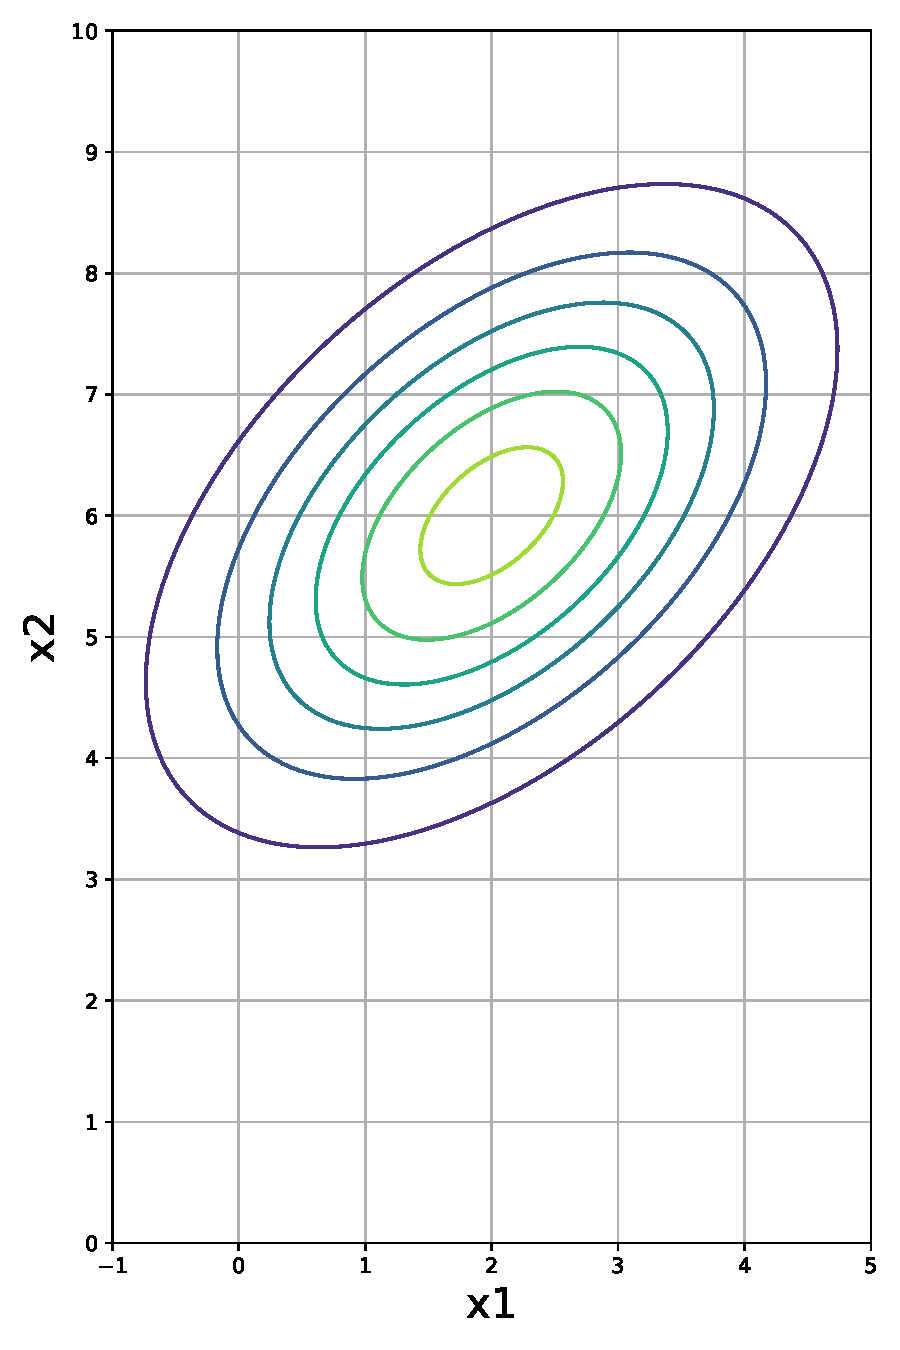
\includegraphics[width=0.5\linewidth]{exercise3_a}
\caption{Gussian random data.}
\label{fig: figure 1}
\end{figure}
\pagebreak
\subsection*{Exercise 4}
Type your third problem here.











\end{document}

